\chapter{Вторая глава. Описание моделей}
\label{cha:ch_2}
\section{Модель раскрытия совместного преступления}
Модель раскрытия совместного преступления, предложенная Спенглером \cite{Spengler}, предполагает игру в развернутой форме для трех игроков с эндогенным характером формирования игровых историй.
Игра построена следующим образом. В игре учавствуют три игрока: клиент(C), чиновник(O) и инспектор(I). Игру начинает клиент. Клиент может подкупить чиновника с вероятностью $\gamma$ или нет с вероятностью $1 - \gamma$. Чиновник, в случае подкупа, может ответить взаимностью с вероятностью $\beta$ или нет с вероятностью $1 - \beta$. Взаимность определяется как акт возврата благосклонности за взятку, то есть возвращение некоторых привелегий (например, государственный контракт) клиенту. Коррупция, как взаимное взяточничество, может произойти только при совместных усилиях клиента и чиновника. Игра включает в себя четыре штрафа, один за подкуп $p_L$ и один для получения взаимности $q_L$ (штрафы клиента), а также один для принятия взятки и взаимности $q$ (штраф чиновника). Это позволяет использовать асимметричное распределение штрафов. Штрафы применяются с вероятностью инспектирования, которая представлена действием инспектора. Таким образом инспектор может провести проверку c вероятностью $\alpha$, либо не проводить с вероятностью $1 - \alpha$. При этом награда инспетора зависит факта инспектирования и наличия преступления. 
\par 
Для подкупа чиновника клиент тратит $b$ на взятку и получает выгоду от взаимности чиновника в размере $v$. Чиновник в случае подкупа получает взятку в размере $b$ , а неотвечая взяимностью получает $r$. Параметр $r$ играет роль нейтральной выплаты, для подкрепления непринятия взятки и может быть расценен как моральное удавлетворение от несовершения преступления. В случаях выявленного преступления клиент и чиновник должны выплатить соответствующие штрафы. 
Распределение выплат инспектору показано в таблице \ref{tbl:inspr1}.
\begin{table}[H]
	\centering
	\begin{tabular}[t]{|c|c|c|}
		\hline
		История игры & Провести проверку: $\alpha$ & Не проводить: $1-\alpha$ \\
		\hline
		Взаимная взятка: $\gamma \beta$ & $x + \Delta x$ & $x$ \\
		\hline
		Невзяимная взятка: $\gamma (1 - \beta$) &  $y + \Delta y$ & $y$ \\
		\hline
		Не было взятки: $(\gamma - 1)$ &  $z$ & $z + \Delta z$ \\
		\hline
	\end{tabular}
	\caption{\centering Схема распределения выплат инспектору}
	\label{tbl:inspr1}
\end{table}
\par
Предполагается, что проверка приводит к лучшим для инспектора результатам в случае (взаимного) взяточничества, чем в случае отсутствия взяточничества и наоборот: $0 <∆x, ∆y, ∆z$.
\par
Для клиента мы предполагаем, что взяточничество является прибыльным, если оно встречает взаимность, но не с проверкой, где $b$ - взятка, а $v$ - это выгода от взаимного обращения с клиентом. Это подразумевает, что $0 < b < v$ и $0 < p_L$, $p_H$ и $v - b - p_L - p_H <0$.
Для инспектора предполагется, что проверка является прибыльной, если по крайней мере один правонарушитель совершает правонарушения, но обходится дорого, если нет. Это подразумевает, что $x <0 <x + ∆x$ и $y <0 <y + ∆y$, но $z <0 <z + ∆z$. Эта настройка отражает интуицию, что успешный осмотр стоит того, поскольку он приводит к продвижению или аналогичным выгодам, в то время как безуспешная проверка просто стоит усилий. Сложность модели требует, чтобы мы сделали некоторые дополнительные предположения о выплатах инспектора. Мы предполагаем, что проверка взаимного взяточничества является более прибыльной, чем проверка простого взяточничества, и, аналогично, что не проверки взаимного взяточничество несет большую потерю, чем не проверка простого взяточничества из-за более высокой альтернативной стоимости неинспекции. Это подразумевает, что $0 <y + ∆y <x + ∆x$ и $x < y < 0$. Для чиновника мы предполагаем, что получение взятки является прибыльным, пока нет проверки, подразумевая, что $0 < r < b < q$.
\par
Последовательность выборов игроков и распределение выплат данной игры могут быть представлены в развернутой форме. Развернутая форма игры представлена на рисунке \ref{fig:figef1}.
\begin{figure}[H]
	\centering
	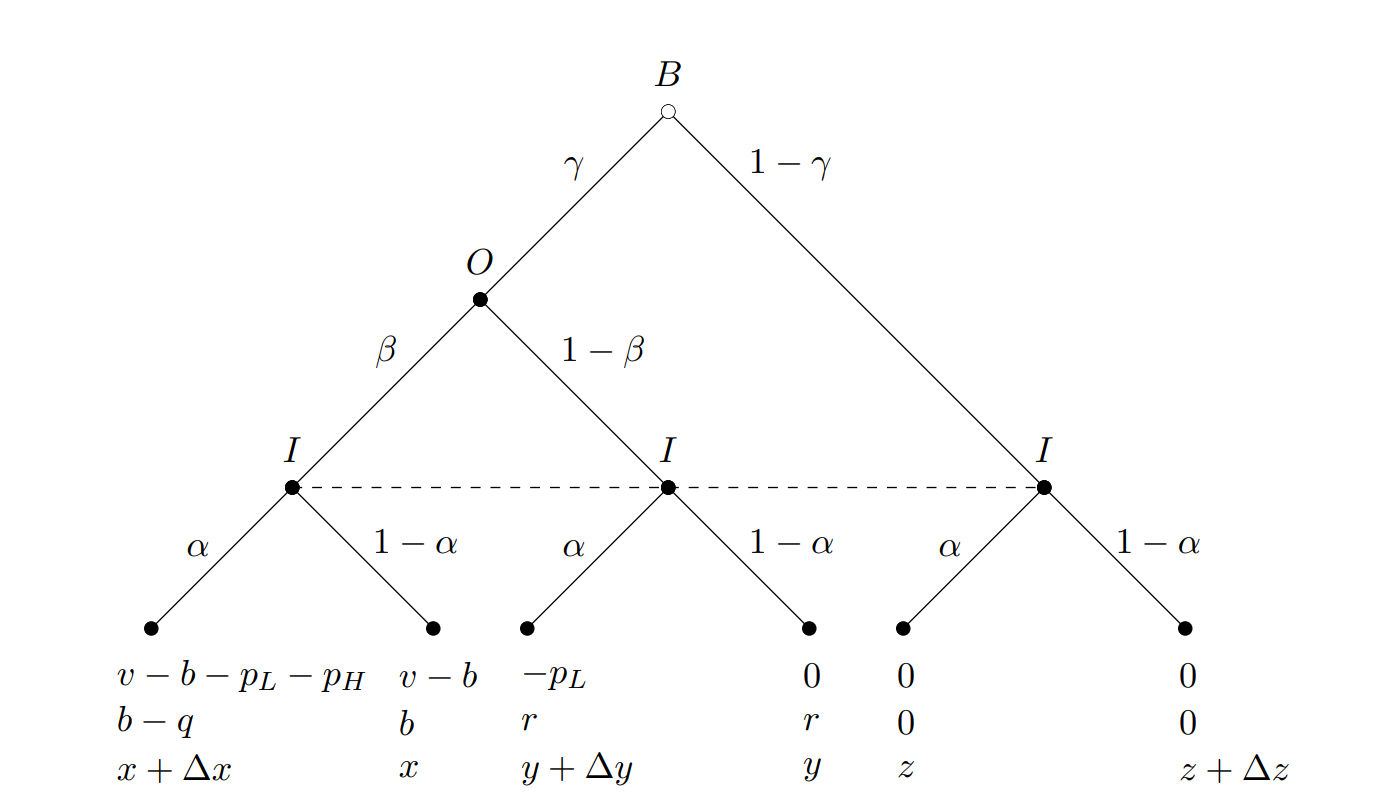
\includegraphics[width=0.9\linewidth]{inc/img/ef1}
	\caption{Развернутая форма игры}
	\label{fig:figef1}
\end{figure}
\par
Рассмотрим равновесие данной игры. Чтобы алгебраически выразить равновесие, для каждого игрока приравняем выплаты каждой стратегии. Используя выплаты на рисунке \ref{fig:figef1}, мы получаем уравнения (\ref{eq:2.1}), (\ref{eq:2.2}) и (\ref{eq:2.3}), связанные с выплатами клиента, чиновника и инспектора соответственно.
\begin{equation}\label{eq:2.1}
	\beta(v-b-\alpha(p_L + p_H)) + (1 - \beta)(-\alpha p_L)=0
\end{equation}
\begin{equation}\label{eq:2.2}
	\alpha(b-q) + (1-\alpha)b=\alpha r + (1-\alpha)r
\end{equation}
\begin{equation}\label{eq:2.3}
	\gamma \beta(x+\Delta x) + \gamma(1-\beta)(y+\Delta y) + (1 - \gamma)z = \gamma \beta x + \gamma(1-\beta)y + (1 - \gamma) (z + \Delta z)
\end{equation}
\par
Мы получаем следующие вероятности равновесия для $v$, $\beta$ и $\alpha$ из предыдущих уравнений:
\begin{equation}\label{eq:2.4}
	\beta = \frac{\alpha p_L}{v - b - \alpha p_H}
\end{equation}
\begin{equation}\label{eq:2.5}
	\alpha = \frac{b - r}{q}
\end{equation}
\begin{equation}\label{eq:2.6}
	\gamma = \frac{\Delta z}{\beta (\Delta x - \Delta y) + \Delta y + \Delta z}
\end{equation}
Дальнейшие преобразования (\ref{eq:2.4}-\ref{eq:2.6}) позволяют получить выражения $\beta$ и $\gamma$ заисящие от параметров:
\begin{equation}\label{eq:2.7}
	\alpha = \frac{(b - r)p_L}{(v - b)q - (b - r)p_H}
\end{equation}
\begin{equation}\label{eq:2.8}
	\gamma = \frac{((v-b)q - (b - r)p_H)\Delta z}{(b-r)p_L(\Delta x - \Delta y) + ((v-b)q-(b-r)p_H)(\Delta y + \Delta z)}
\end{equation}
\par
Относительно полученных значений можно отметить следующие предположения:
\begin{itemize}
	\item для клиента вероятность предложения взятки должна быть равна нулю, если вероятность принятия меньше вероятности принятия/возврата в уравнении (\ref{eq:2.4}) и равна одному в обратном случае;
	\item для чиновника вероятность принятия должна быть равна нулю, если вероятность проверки больше, чем вероятность проверки в уравнении (\ref{eq:2.5}) и равен одному в обратном случае;
	\item для инспектора вероятность проверки должна быть равна нулю, если вероятность предложения взятки меньше, чем вероятность предложения взятки в уравнении(\ref{eq:2.6}) и равна единице в обратном случае.
\end{itemize}
\par
Помимо приведенного выше примера, также рассматривается вариант данной игры, в котором не проводится проверка после отклонения взятки, а сразу выписывается штраф \cite{Spengler}. Но в силу того, что проверка коррупции часто инициируется заранее, то факт проверки часто не зависит от факта предложения взятки. Таким образом ограничемся только этим более обобщенным вариантом.
\section{Модель коррупции в иерархической структуре}
Орлов\cite{Orlov} предложил иерархическую модель коррупции для отражения дополнительной связи между руководителями и подчиненными. В данной работе возьмем за основу эту модель, но, как и в прошлом примере, попробуем эндогенезировать действия игроков.
Коррупция моделируется как иерархическая игра, которая состоит из двух стадий: кража и проверка. Предполагается, что игроки действуют из соображений нейтрального риска и максимизации личного выигрыша. Рассматриваются только денежные выплаты. Модель предполагает, что иерархия клиентов представляет из себя древовидную структуру, в которой от корня к вершинам ведут связи от начальника к подчиненному.
Зададим иерархию клиентов следующими элементами:
\begin{itemize}
\item Конечное множество различных сотрудников $C$;
\item $s\colon C\to R$ "--- сумма средств, которую сотрудник может присвоить себе не прекращая производственный процесс;
\item $b\colon C\to R$ "--- размер взятки, которую сотрудник готов предложить проверяющему чиновнику;
\item $d\colon C\to C$ "--- руководитель сотрудника. В случае, если  $b(c) = c$, то $c$ не имеет руководства.
 
\end{itemize}
Будем придерживаться следующих ограничений: $\forall c \in C\;\;0 < b(c) < s(c)$, $s(c) < s(d(c))$, если $b(c) \neq c$ и $d(c1)=d(c2) =>s(c1)=s(c2)$. Таким образом, взятка не может превосходить украденную сумму, а подчиненный не может располагать большей суммой, чем руководитель. Данные ограничения соответствуют концепции нейтрального риска\cite{Orlov}.
Помимо каждого сотрудника из иерархии, в игре участвуют еще 2 игрока: чиновник ($O$) и инспектор ($I$). Чиновник может провести проверку сотрудников, а инспектор может проверить факт получения взятки чиновником. Саму игру разобьем на три этапа. Gроверенный сотрудник может выплатить штраф, подкупить чиновника, либо разоблачить руководителя.
Для формирования выплат игроков введем дополнительные параметры:
\begin{itemize}
	\item $co$ "--- стоимость проверки сотрудника;
	\item $ci$ "--- стоимость проверки инспектора;
	\item $fs$ "--- размер штрафа, который сотрудник должен выплатить за выявленную кражу;
	\item $fb$ "--- размер штрафа, который сотрудник получает за предложение взятки;
	\item $fq$ "--- размер штрафа, который получает чиновник за получение взятки;
	\item $fns$ "--- штраф чиновника за каждую совершенную кражу;
	\item $fe$ "--- штраф за ложный донос;
	\item $fbc$ "--- размер штрафа инспектору за непроверенную взятку чиновника;
	\item $rs$ "--- награда, которую чиновник получает за выявленную кражу;
	\item $rb$ "--- награда, которую чиновник получает за отклонение взятки;
	\item $rq$ "--- награда, которую получает инспектор за выявленную взятку чиновника.
\end{itemize}
На первом этапе инспектор может инициировать проверку чиновника, либо не инициировать. Он начинает первым, по причине того, что факт получения взятки редко доказывается косвенно, и проверки часто связаны с прослушкой и подставными агентам, что должно быть организовано заранее.
\par
На втором этапе компания выделяет сумму сотрудникам, так, что каждый сотрудник $c \in C$ имеет возможность присвоить $s(c)$. Затем, каждый сотрудник $c$ может совершить кражу в размере $s(c)$ или не совершать. Обозначим за $S_c$ обьем кражи сотрудника c, которую он совершил на данном этапе. $S_c = 0$ , если сотрудник c не совершал кражу.
\par
На третьем этапе чиновник принимает решение о проверке одного из сотрудников. В некоторых предыдущих работах \cite{Orlov}, предполагается, что проверка проводится с вероятностью, которая зависит от объема краж всех вышестоящих сотрудников. Но в данной работе такой подход не рассматривается, и чиновник самостоятельно принимает решение. Чиновник может и вовсе не проводить проверку. Проверенного сотрудника обозначим как $c_{insp}$. Если проверка не проводилась или если $S_{c_{insp}}$ = 0, то игра заканчивается, и игроки получают свои выплаты. 
В случае, если $S_{c_{insp}} > 0$, игра продолжается и $c_{insp}$ может выбрать одну из следующих альтернатив:
\begin{itemize}
	\item признать свое преступление и выплатить штраф $fs$;
	\item предложить чиновнику взятку в размере $b(c_{insp})$, в обмен на сокрытие своей кражи;
	\item попытаться разоблачить руководителя. 
\end{itemize}
Разоблачение руководителя аналогично его проверке, с той разницей, что сдавший его подчиненный, в случае выявленной кражи руководителя, не платит штраф за кражу. Однако, если разоблаченный руководитель не совершил кражу, то сдавший его подчиненный выплачивает свой штраф за кражу и получает дополнительный штраф за ложный донос.
\par 
Если сотрудник предложил взятку, инспектор может либо принять взятку, либо отклонить. Если чиновник принимает взятку, то он получает ее сумму, если не инициирована проверка инспектором, а клиенты сохраняют украденное. Если чиновник берет взятку во время проверки инспектором, то он не получает сумму взятки и должен выплатить штраф, а сотрудник получает ту же выплату, что и в случае отклонения взятки. В случае отклонения взятки сотрудник выплачивает штрафы, и за взятку, и за кражу. При этом, если инспектор не принимает взятку, то все проверенные сотрудники возвращают украденное.
\par
Для наглядной иллюстрации применения всех этих правил рассмотрим один пример.
Возьмем иерархию из двух сотрудников, один будет подчиняться другому.
	$$C = \{C_0, C_1\},$$
	$$s(C_0) = s_0,$$
	$$s(C_1) = s_1,$$
	\begin{equation}\label{eq2.9} b(C_0) = b_0,\end{equation}
	$$b(C_1) = b_1,$$
	$$d(C_0) = d(C_1) = C_0.$$

Тогда в игре будут участвовать 4 игрока: сотрудник 0, сотрудник 1, чиновник и инспектор. Схематичное изображение развернутой формы этой игры представлено на рисунках \ref{fig:figef21} и \ref{fig:figef22}. Изображение разбито на 2 части, в зависимости от выбора инспектора.
\begin{figure}[H]
	\centering
	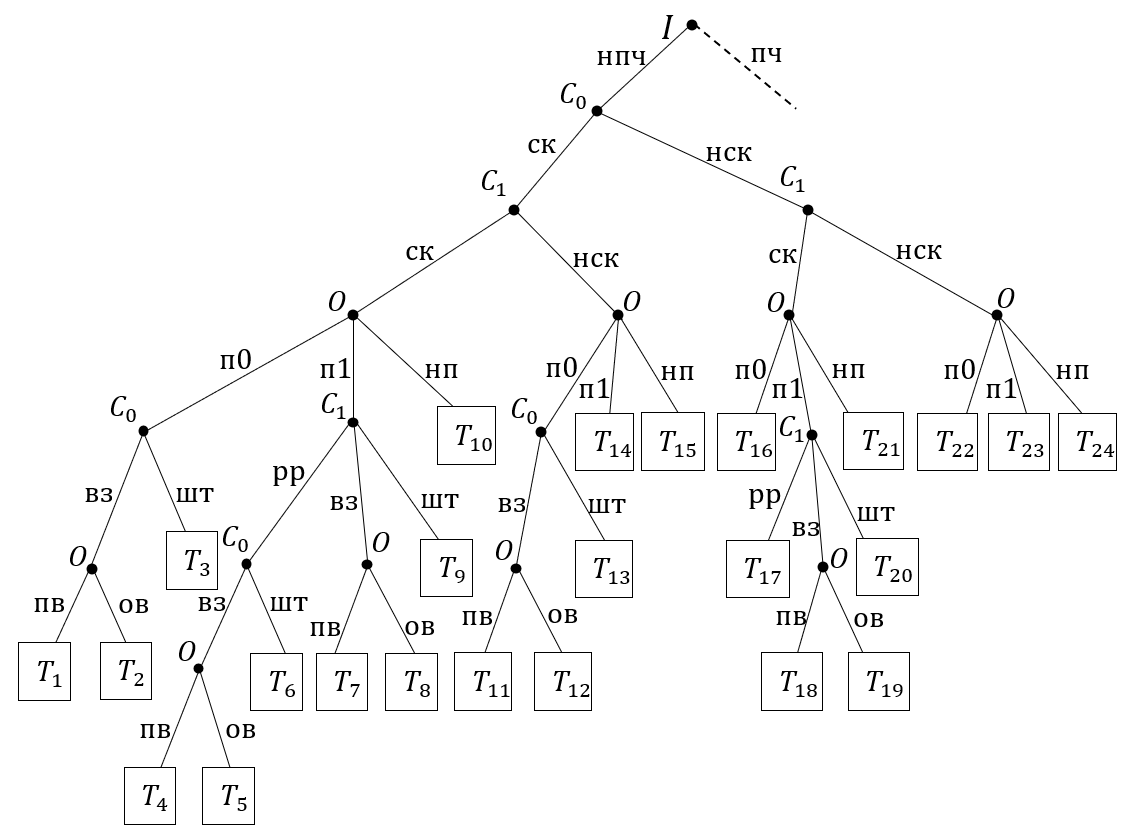
\includegraphics[width=0.9\linewidth]{inc/img/ef21}
	\caption{Развернутая форма игры. Часть 1}
	\label{fig:figef21}
\end{figure}
\begin{figure}[H]
	\centering
	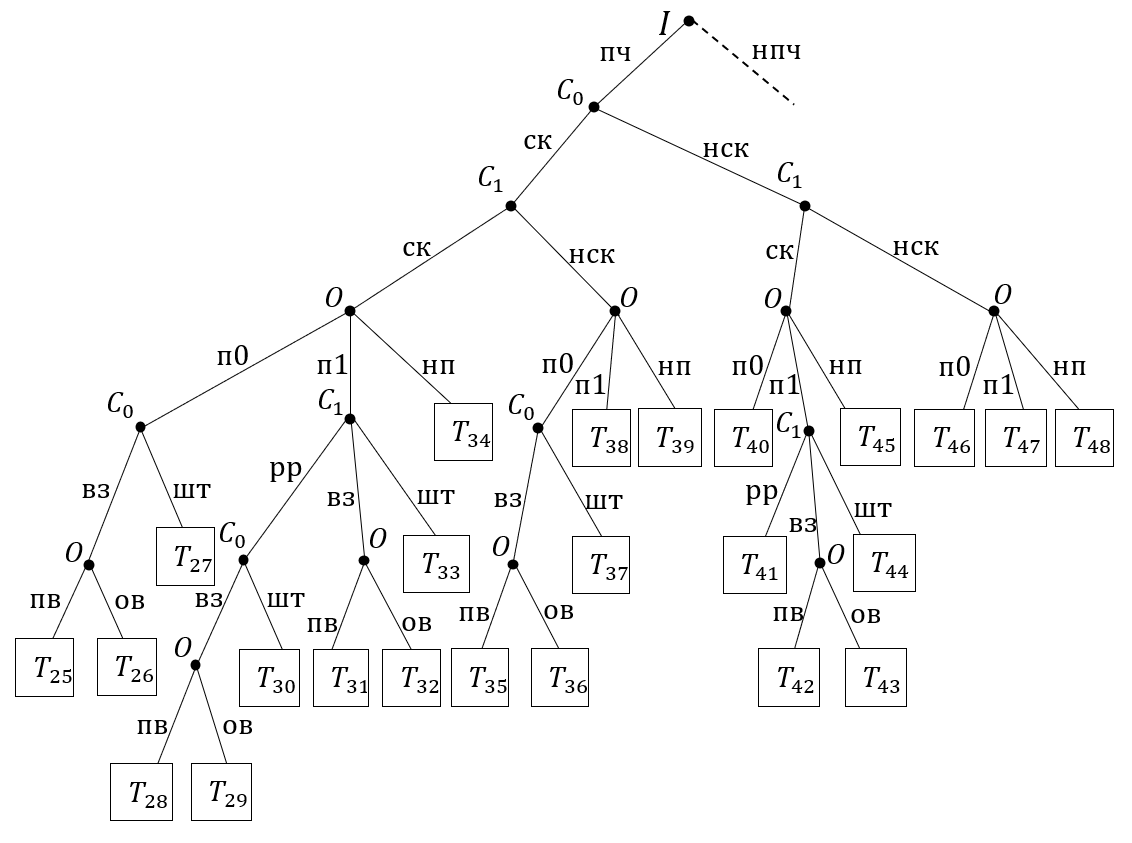
\includegraphics[width=0.9\linewidth]{inc/img/ef22}
	\caption{Развернутая форма игры. Часть 2}
	\label{fig:figef22}
\end{figure}
\par
На рисунках \ref{fig:figef21} и \ref{fig:figef22} возле ребер подписаны соответствующие им действия. Их можно расшифровать так:
\begin{itemize}
	\item $\text{пч}$ "--- проверять чиновника;
	\item $\text{нпч}$ "--- не проверять чиновника;
	\item $\text{ск}$ "--- совершить кражу;
	\item $\text{нск}$ "--- не совершать кражу;
	\item $\text{п0}$ "--- проверить сотрудника $C_0$;
	\item $\text{п1}$ "--- проверить сотрудника $C_1$;
	\item $\text{нп}$ "--- не проверять сотрудников;
	\item $\text{рр}$ "--- разоблачить руководителя;
	\item $\text{вз}$ "--- предложить взятку;
	\item $\text{шт}$ "--- выплатить штраф;
	\item $\text{пв}$ "--- принять взятку;
	\item $\text{ов}$ "--- отклонить взятку.
\end{itemize}
\par
На рисунках \ref{fig:figef21} и \ref{fig:figef22} буквами $T$ обозначены все 48 различных выплат в терминальных узлах. Ниже представлены величины этих выплат.
\par
\begin{align*}
	T_1 = & (s_0-b_0, s_1, b_0- 2 * fns - co,-fbc) \\
	T_2 = &(-b_0-fs-fb, s_1, rs + rb-fns - co, 0) \\
	T_3 = &(-b_0-fs, s_1, rs-fns - co, 0) \\
	T_4 = &(s_0-b_0, s_1, b_0 - fns * 2 - co, -fbc) \\
	T_5 = &(-b_0-fs - fb, 0, rs * 2 + rb - co, 0) &
	T_6 = &(-fs, 0, rs * 2 - co, 0) \\
	T_7 = &(s_0, s_1-b_1, b_1-fns * 2 - co, -fbc) \\
	T_8 = &(s_0, -b_1 -fs -fb, rs + rb - fns - co, 0) \\
	T_9 = &(s_0, -fs, rs - co, 0) &
	T_{10} =& (s_0, s_1, -fns * 2, 0) \\
	T_{11} = &(s_0-b_0, 0, b_0-fns - co, -fbc) &
	T_{12} = &(-b_0-fs-fb, 0, rs + rb - co, 0) \\
	T_{13} = &(-fs, 0, rs - co, 0) &
	T_{14} = &(s_0, 0, -fns - co, 0) \\
	T_{15} = &(s_0, 0, -fns, 0) &
	T_{16} = &(0, s_1, -fns - co, 0) \\
	T_{17} = &(0, -fs-fe, rs-co, 0) &
	T_{18} = &(0, s_1-b_1, b_1-fns-co, -fbc) \\
	T_{19} = &(0,-b_1 -fs-fb, rs + rb - co, 0) &
	T_{20} = &(0, -fs, rs, 0) \\
	T_{21} = &(0, s_1, -fns, 0) &
	T_{22} = &(0, 0, -co, 0) \\
	T_{23} = &(0, 0, -co, 0) &
	T_{24} = &(0, 0, 0, 0) \\
	T_{25} = &(-b_0-fs -fb, s_1, fq-fns * 2-co, rq -ci) \\
	T_{26} = &(-b_0-fs-fb, s_1, rs + rb-fns - co, -ci) \\
	T_{27} = &(-fs, s_1, rs-fns-co, -ci) &
	T_{28} = &(-fs-fb, 0, fq-co, rq-ci) \\
	T_{29} = &(-fs-fb, 0, rs * 2 + rb-co, -ci) &
	T_{30} = &(-fs, 0, rs * 2-co, ci) \\
	T_{31} = &(s_0, -b_1 -fs-fb, fq-fns-co, rq-ci) \\
	T_{32} = &(s_0, -b_1 -fs-fb, rs + rb-fns - co, -ci) \\
	T_{33} = &(s_0, -fs, rs - co, -ci) &
	T_{34} = &(s_0, s_1, -fns * 2, -ci) \\
	T_{35} = &(-b_0-fs-fb, 0, fq-co, rq -ci) \\
	T_{36} = &(-b_0-fs-fb, 0, rs + rb - co, -ci) \\
	T_{37} = &(-fs, 0, rs - co, -ci) &
	T_{38} = &(s_0, 0, -fns - co, -ci) \\
	T_{39} = &(s_0, 0, -fns, -ci) &
	T_{40} = &(0, s_1, -fns - co, -ci) \\
	T_{41} = &(0, -fs-fe, rs-co, -ci) \\
	T_{42} = &(0, -b_1 -fs-fb, fq - co, rq -ci) \\
	T_{43} = &(0, -b_1 -fs-fb, rs + rb - co, -ci) &
	T_{44} = &(0, -fs, rs, -ci) \\
	T_{45} = &(0, s_1, -fns, -ci) &
	T_{46} = &(0, 0, -co, -ci) \\
	T_{47} = &(0, 0, -co, -ci) &
	T_{48} = &(0, 0, 0, -ci)	
\end{align*}
